\documentclass[tikz,border=14pt]{standalone}
\usepackage[T1]{fontenc}
\usepackage{tgheros}
\renewcommand*\familydefault{\sfdefault}
\usepackage{pgfplots}
\pgfplotsset{compat=1.18}
\usepgfplotslibrary{fillbetween}
\usetikzlibrary{arrows.meta, calc}
\pgfdeclarelayer{background}
\pgfsetlayers{background,main}
\newcommand{\toyCliffA}{99.9000}\newcommand{\toyCliffAL}{99.9}
\newcommand{\toyCliffB}{71.5000}\newcommand{\toyCliffBL}{71.5}
\newcommand{\toyCliffC}{3.6667}\newcommand{\toyCliffCL}{3.7}
\newcommand{\toyCliffD}{1.6333}\newcommand{\toyCliffDL}{1.6}
\newcommand{\realCliffA}{84.5000}\newcommand{\realCliffAL}{84.5}
\newcommand{\realCliffB}{51.0000}\newcommand{\realCliffBL}{51.0}
\newcommand{\realCliffC}{6.5000}\newcommand{\realCliffCL}{6.5}
\newcommand{\toyAttA}{0.7122}\newcommand{\toyAttAL}{0.71}
\newcommand{\toyAttB}{0.4090}\newcommand{\toyAttBL}{0.41}
\newcommand{\toyAttC}{0.1179}\newcommand{\toyAttCL}{0.12}
\newcommand{\toyAttD}{0.0241}\newcommand{\toyAttDL}{0.02}
\newcommand{\realAttIn}{0.4632}\newcommand{\realAttInL}{0.46}
\newcommand{\realAttFar}{0.1077}\newcommand{\realAttFarL}{0.11}
\newcommand{\realHeads}{39.0000}\newcommand{\realHeadsL}{39}
\newcommand{\toyNone}{1.6667}\newcommand{\toyNoneL}{1.7}
\newcommand{\realTwoNone}{51.0000}\newcommand{\realTwoNoneL}{51.0}
\newcommand{\realFourNone}{6.5000}\newcommand{\realFourNoneL}{6.5}
\newcommand{\toyPatch}{76.1500}\newcommand{\toyPatchL}{76.1}
\newcommand{\realTwoPatch}{85.5000}\newcommand{\realTwoPatchL}{85.5}
\newcommand{\realFourPatch}{65.0000}\newcommand{\realFourPatchL}{65.0}
\newcommand{\toySham}{1.2833}\newcommand{\toyShamL}{1.3}
\newcommand{\realTwoSham}{1.0000}\newcommand{\realTwoShamL}{1.0}
\newcommand{\realFourSham}{1.0000}\newcommand{\realFourShamL}{1.0}
\newcommand{\realFourPatchFull}{25.5000}\newcommand{\realFourPatchFullL}{25.5}
\newcommand{\bestFixAnywhere}{9.3333}\newcommand{\bestFixAnywhereL}{9.3}
\newcommand{\fixMaxFar}{1.4333}\newcommand{\fixMaxFarL}{1.4}
\newcommand{\auditToyNone}{1.5833}\newcommand{\auditToyNoneL}{1.6}
\newcommand{\auditToyPatch}{75.6667}\newcommand{\auditToyPatchL}{75.7}
\newcommand{\auditTwoNone}{55.5556}\newcommand{\auditTwoNoneL}{55.6}
\newcommand{\auditTwoPatch}{100.0000}\newcommand{\auditTwoPatchL}{100.0}
\newcommand{\auditTwoN}{18.0000}\newcommand{\auditTwoNL}{18}
\newcommand{\marginOrig}{0.6780}\newcommand{\marginOrigL}{0.68}
\newcommand{\marginAudit}{1.1240}\newcommand{\marginAuditL}{1.12}


\definecolor{ink}{HTML}{0B0B0B}
\definecolor{muted}{HTML}{6B6A66}
\definecolor{gridc}{HTML}{E6E5E0}
\definecolor{band}{HTML}{F3F2EE}
\definecolor{cnone}{HTML}{52514E}
\definecolor{cpatch}{HTML}{2A78D6}
\definecolor{csham}{HTML}{008300}
\definecolor{corange}{HTML}{EB6834}
\definecolor{softblue}{HTML}{CFE1F7}
\definecolor{softgray}{HTML}{C9C8C2}

\newcommand{\pct}[1]{#1\%}

\pgfplotsset{
  /pgf/number format/assume math mode=true,
  base/.style={
    axis line style={muted, line width=0.4pt},
    tick style={muted, line width=0.4pt},
    tick align=outside,
    axis x line*=bottom, axis y line*=left,
    every tick label/.append style={font=\small, text=muted},
    label style={font=\small, text=muted},
    grid=major, major grid style={gridc, line width=0.4pt},
    title style={font=\normalsize\bfseries, text=ink},
    clip=false,
  },
}
\tikzset{
  figtitle/.style={font=\LARGE\bfseries, text=ink, anchor=north west, inner sep=0pt},
  figsub/.style={font=\normalsize, text=muted, anchor=north west, align=left, text width=17cm, inner sep=0pt, execute at begin node={\hyphenpenalty=10000\exhyphenpenalty=10000}},
  footnote/.style={font=\small, text=muted, anchor=north west, align=left, text width=17cm, inner sep=0pt, execute at begin node={\hyphenpenalty=10000\exhyphenpenalty=10000}},
  big/.style={font=\Large\bfseries, inner sep=2pt},
  lab/.style={font=\small, text=ink, inner sep=2pt},
  quiet/.style={font=\small, text=muted, inner sep=2pt},
}
\newcommand{\header}[2]{\node[figtitle] (title) at (0,0) {#1};
  \node[figsub] (sub) at ($(title.south west)+(0,-8pt)$) {#2};}

\newcommand{\ax}[1]{(5.6 + 0.115*(#1))}
\newcommand{\rescue}[5]{\draw[#4, line width=3.4pt, -{Stealth[length=11pt, width=12pt]}] ({\ax{#2} + 0.12}, #1) -- ({\ax{#3}}, #1);
  \fill[#4, draw=white, line width=1pt] ({\ax{#2}}, #1) circle (3.6pt);
  \node[lab, font=\normalsize\bfseries, text=#4, anchor=west] at ({\ax{#3} + 0.12}, #1) {#5};}
\begin{document}
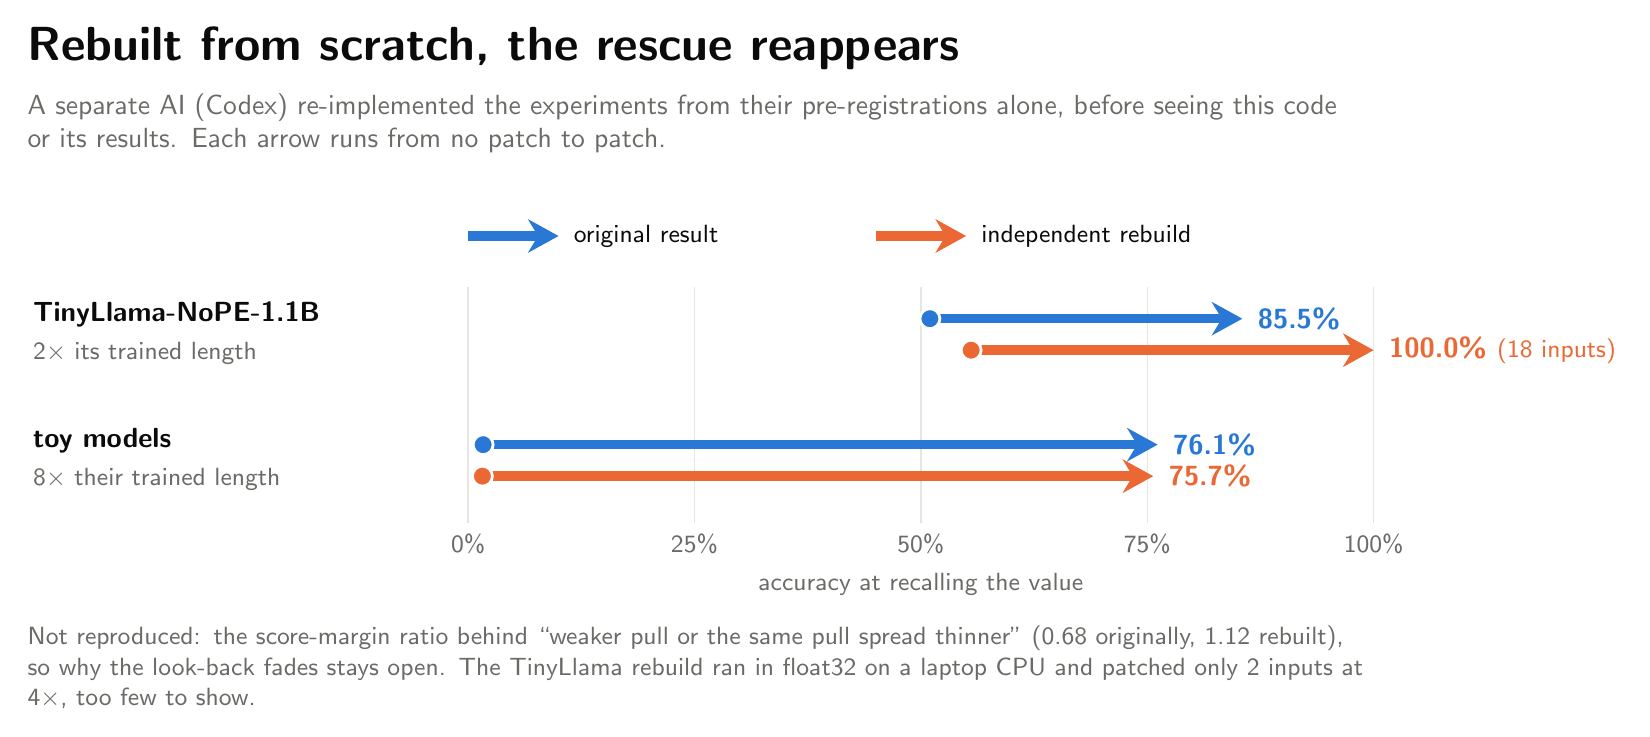
\begin{tikzpicture}
  \header{Rebuilt from scratch, the rescue reappears}
    {A separate AI (Codex) re-implemented the experiments from their pre-registrations alone, before seeing this
     code or its results. Each arrow runs from no patch to patch.}

  \begin{scope}[shift={($(sub.south west)+(0,-2.3cm)$)}]
    \draw[cpatch, line width=3.4pt, -{Stealth[length=11pt, width=12pt]}] ({\ax{0}}, 1.25) -- ({\ax{10}}, 1.25);
    \node[lab, anchor=west] at ({\ax{11}}, 1.25) {original result};
    \draw[corange, line width=3.4pt, -{Stealth[length=11pt, width=12pt]}] ({\ax{45}}, 1.25) -- ({\ax{55}}, 1.25);
    \node[lab, anchor=west] at ({\ax{56}}, 1.25) {independent rebuild};

    \foreach \a in {0,25,50,75,100} {
      \draw[gridc, line width=0.5pt] ({\ax{\a}}, 0.6) -- ({\ax{\a}}, -2.4);
      \node[quiet, anchor=north] at ({\ax{\a}}, -2.45) {\a\%};
    }
    \node[quiet, anchor=north] at ({\ax{50}}, -2.95) {accuracy at recalling the value};

    \node[lab, font=\normalsize\bfseries, anchor=south west] at (0, 0.02) {TinyLlama-NoPE-1.1B};
    \node[quiet, anchor=north west] at (0, -0.02) {2$\times$ its trained length};
    \rescue{0.2}{\realTwoNone}{\realTwoPatch}{cpatch}{\pct{\realTwoPatchL}}
    \rescue{-0.2}{\auditTwoNone}{\auditTwoPatch}{corange}{\pct{\auditTwoPatchL}
      \textmd{\small (\auditTwoNL{} inputs)}}

    \node[lab, font=\normalsize\bfseries, anchor=south west] at (0, -1.58) {toy models};
    \node[quiet, anchor=north west] at (0, -1.62) {8$\times$ their trained length};
    \rescue{-1.4}{\toyNone}{\toyPatch}{cpatch}{\pct{\toyPatchL}}
    \rescue{-1.8}{\auditToyNone}{\auditToyPatch}{corange}{\pct{\auditToyPatchL}}
  \end{scope}

  \node[footnote] at ($(sub.south west)+(0,-6.0cm)$) {Not reproduced: the score-margin ratio behind ``weaker
    pull or the same pull spread thinner'' (\marginOrigL{} originally, \marginAuditL{} rebuilt), so why the
    look-back fades stays open. The TinyLlama rebuild ran in float32 on a laptop CPU and patched only 2 inputs at
    4$\times$, too few to show.};
\end{tikzpicture}
\end{document}
